% Alicja Jurasik
Na podstawie specyfikacji dokonano rozeznania dost�pnych na rynku czujnik�w odleg�o�ci. Odrzucono sensory cyfrowe ze wzgl�du na to, �e nie zwracaj� informacji o odleg�o�ci do obiektu. Wybieraj�c czujniki analogowe kierowano si� pr�dko�ci� z jak� dokonuj� pomiaru. Dodatkowo podczas selekcji czujnik�w istotny by� zakres prawid�owego dzia�ania, cena oraz waga. Wyniki rozeznania dost�pnych sensor�w przedstawiono w tabeli \ref{tab:czujniki}.
(((((obrazki mia�y by� u�o�one �adnie w jednym wierszu, ale w raporcie zbiorczym nie chce si� to kompilowa�)))))

\begin{figure}[tp] \centering
        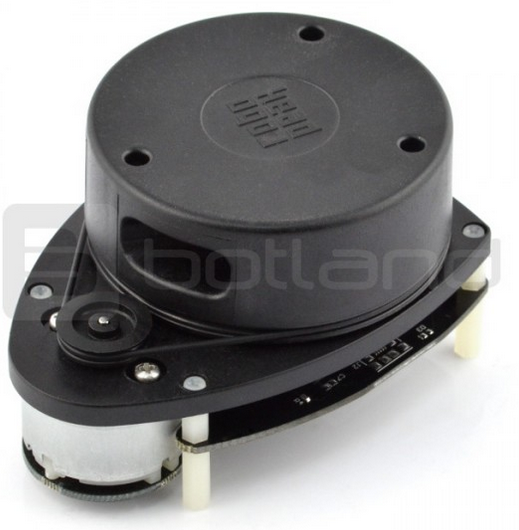
\includegraphics[width=0.18\textwidth]{./grafika/czujnik1.PNG}
        \caption{skaner}
        \label{fig:cz1}
\end{figure}
\begin{figure}[tp] \centering
        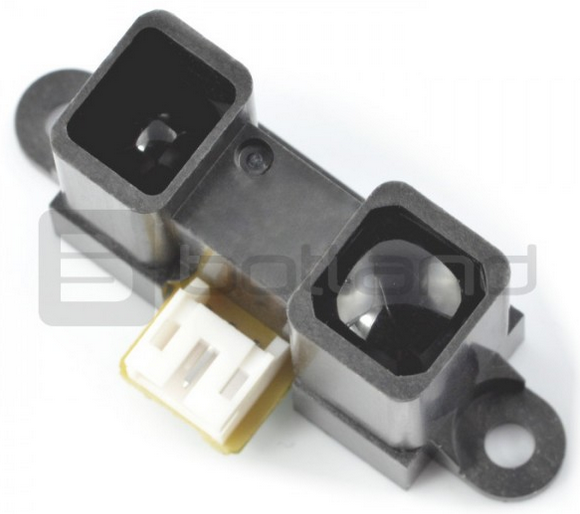
\includegraphics[width=0.18\textwidth]{./grafika/czujnik2.PNG}
        \caption{SHARP}
        \label{fig:cz2}
\end{figure}
\begin{figure}[tp] \centering
        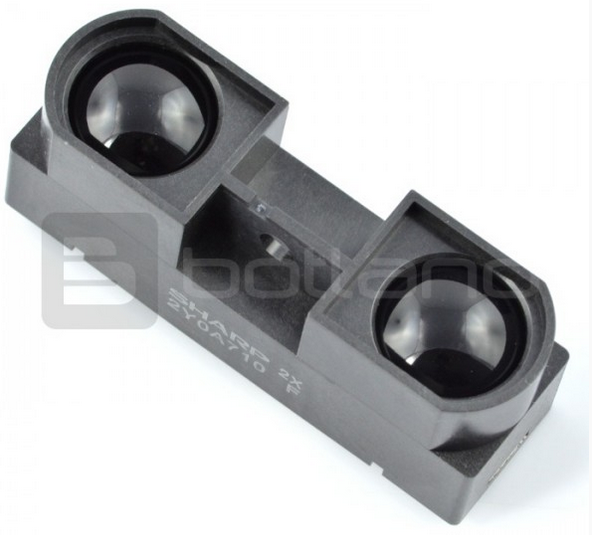
\includegraphics[width=0.18\textwidth]{./grafika/czujnik3.PNG}
        \caption{SHARP}
        \label{fig:cz3}
\end{figure}
\begin{figure}[tp] \centering
        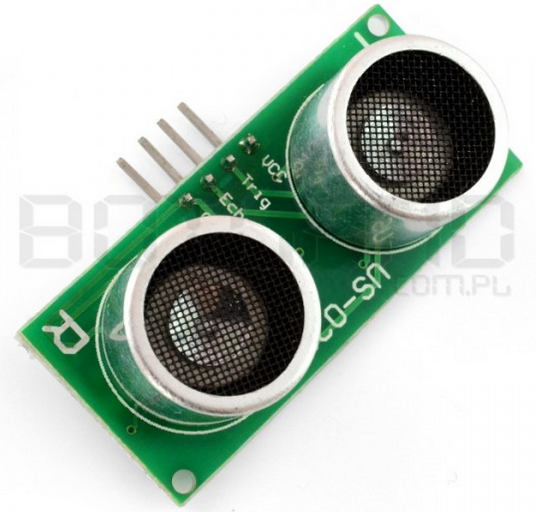
\includegraphics[width=0.18\textwidth]{./grafika/czujnik4.PNG}
                        \caption{sonar}
        \label{fig:cz4}
\end{figure}
\begin{figure}[tp] \centering
        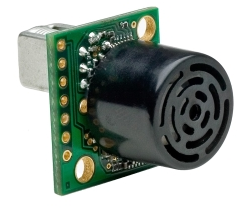
\includegraphics[width=0.18\textwidth]{./grafika/czujnik5.PNG}
                        \caption{sonar}
        \label{fig:cz5}
\end{figure}
%\begin{figure}[h]
%        \centering
%        \begin{subfigure}[b]{0.18\textwidth}{it}
%                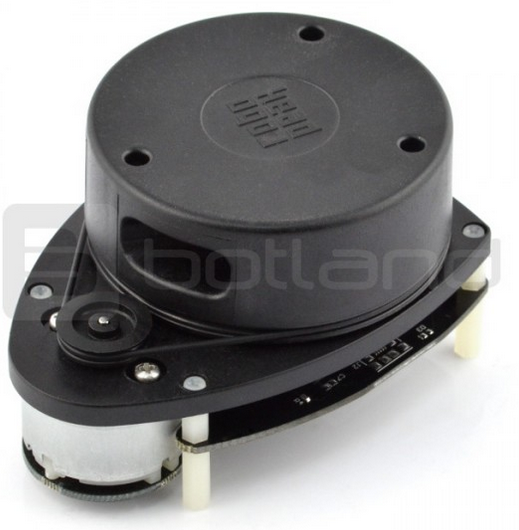
\includegraphics[width=\textwidth]{./grafika/czujnik1.PNG}
%                \caption{cz. laserowy}
%                \label{fig:cz1}
%        \end{subfigure}
%        ~\\
%        \begin{subfigure}[b]{0.18\textwidth}{it}
%                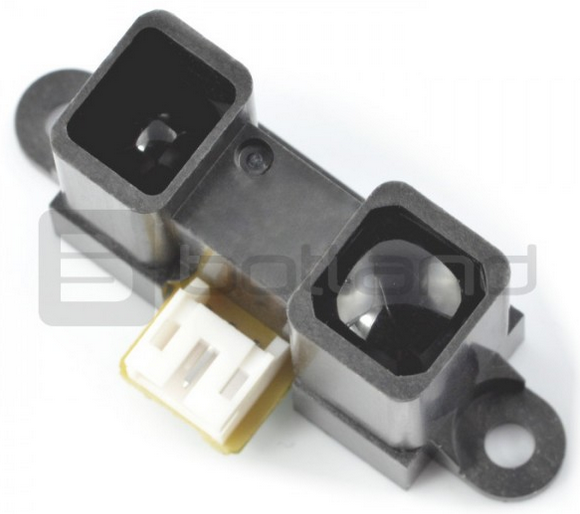
\includegraphics[width=\textwidth]{./grafika/czujnik2.PNG}
%                \caption{SHARP}
%                \label{fig:cz2}
%        \end{subfigure}
%        ~\\
%        \begin{subfigure}[b]{0.18\textwidth}{it}
%                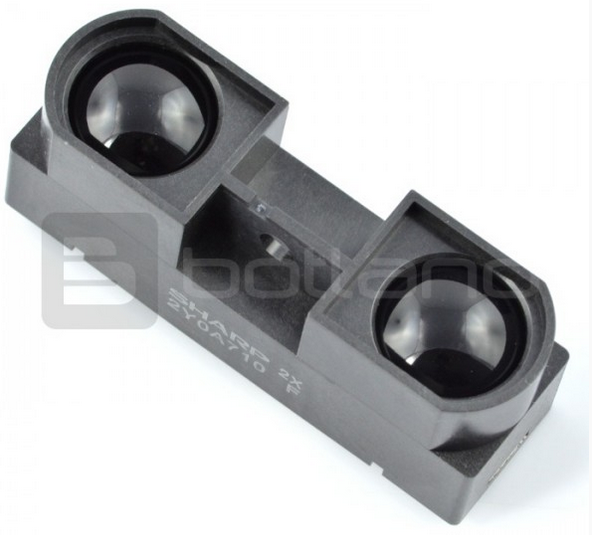
\includegraphics[width=\textwidth]{./grafika/czujnik3.PNG}
%                                \caption{SHARP}
%                \label{fig:cz3}
%        \end{subfigure}
%        ~\\
%        \begin{subfigure}[b]{0.18\textwidth}{it}
%                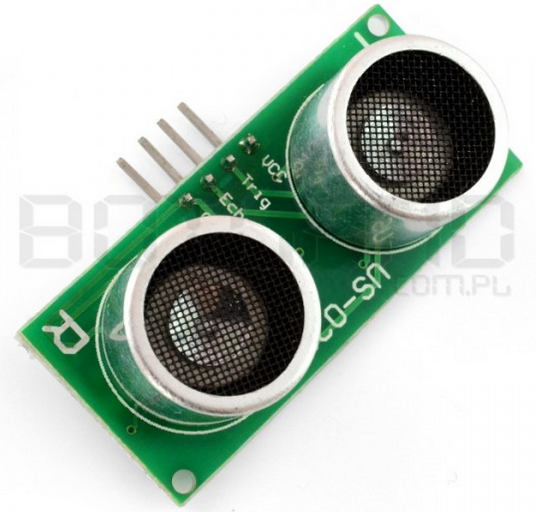
\includegraphics[width=\textwidth]{./grafika/czujnik4.PNG}
%                                \caption{sonar}
%                \label{fig:cz4}
%        \end{subfigure}
%        \\
%        \begin{subfigure}[b]{0.18\textwidth}{it}
%                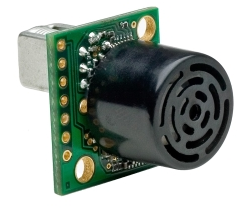
\includegraphics[width=\textwidth]{./grafika/czujnik5.PNG}
%                                \caption{sonar}
%                \label{fig:cz5}
%        \end{subfigure}       
%
%        \caption{Obrazy dost�pnych czujnik�w odleg�o�ci}\label{fig:czujniki}
%\end{figure}
\begin{table}
	\caption{Zestawienie dost�pnych na rynku czujnik�w spe�niaj�cych za�o�enia}
	\label{tab:czujniki}
	
	\begin{tabular}{|l|l|c|c|c|c|}
	\hline 
	no�nik energii & czujnik & cena [z�]  & zasi�g [m] & waga [g] & zdj�cie \\  \hline
	laser& skaner laserowy RPLidar & 1870 & 6 & - & \ref{fig:cz1}		\\ \hline
	podczerwie�  & Sharp GP2Y0A02YK0F & 59 & 0,2 - 1,5	& 4,8 & \ref{fig:cz2}\\ \hline
	podczerwie�  & Sharp GP2Y0A710K0F & 139 & 1 - 5,5	& 10 & \ref{fig:cz3}\\ \hline
	ultrad�wi�ki & US-020& 16 & 0,02 - 7 & - &\ref{fig:cz4} \\ \hline
	ultrad�wi�ki & XL-MaxSonar-EZL0& 169 & 10 & 8 & \ref{fig:cz5}\\ \hline
	\end{tabular}
\end{table}
